\section{Results}
\label{sec:results}

\subsection{Setup}
\label{sec:setup}

The instance is a $5\times5$ grid of $M=25$ communities drawn from Austin, TX, each
carrying an ambient level of \SI{45}{\dBA} (8 tiles), \SI{55}{\dBA} (12) or
\SI{65}{\dBA} (5). Three tiles host vertiports --- an airport, a downtown core and an
exurban commuter town --- and traffic runs in both directions on all three
origin--destination pairs. The per-aircraft source level is \SI{45}{\dBA} and one
timestep is \SI{180}{\second}. Fleet size is set by a demand factor, giving the ladder
$N \in \{6,8,14,16,22,24,30,32\}$.

We compare six conditions at every size: the five principles, and a \emph{baseline} ---
the same fleet with the caps opened and every objective cleared, which is the
shortest-time routing the solver returns when no principle has been selected. It is the
zero against which everything here is measured.

\paragraph{The operating point, and why it is not the default} The cap, the protected set
and the objective encoding are set so that each principle constrains the routing on the
fleet range studied. The cap is $D=\SI{6}{\dB}$ of added noise, applied to all five
principles so they face one hard constraint and differ only in their objective; the
Prioritarian protected set is the three busiest non-vertiport communities that are also
low-income. Both choices are forced. At the settings the system ships with --- $D=10$,
and a protected set chosen as the loudest tiles --- the caps sit at a third of the
capacity they allow, and the protected set carries \emph{zero} aircraft-timesteps at every
fleet size, so its objective is satisfied without the routing changing at all. In that
regime Equal and Sufficientarian return the baseline's routing exactly at $N=8$ and
differ from it by less than the solver's own indifference above.
Choosing an operating point at which a principle does something is a precondition for
measuring what it does, not a result.

Utilitarian and Proportional run the count-weighted form of their objectives
(Section~\ref{sec:encoding}), which the solver already exposes. The decibel form does not
prove optimality above $N=8$ on any budget we gave it; the count form proves every cell
we ran, faster by $51\times$ at $N=8$ for Utilitarian and $1110\times$ for Proportional.
That difference belongs to the encoding, not to the principle, and
Section~\ref{sec:tractability} returns to it.

\paragraph{Every cell is four solves} A single solve is one draw from a set of
equally-optimal routings, and which member comes back is decided by the order the
aircraft happen to be listed in. Every cell here is therefore solved four times under
four permutations of that list. A permutation leaves the fleet, the origin--destination
pairs and the feasible set identical, so the spread across the four is the solver's
indifference and nothing else. The permutation at index $k$ is the same for every
condition, so comparisons at fixed $k$ are paired.

That spread is drawn as a band on every curve, and it fixes what counts as a finding: a
difference between two conditions is reported only when their means differ by more than
the larger of their two bands \emph{and} the bands do not overlap. Differences inside the
band are stated as within the tie-break and nothing is built on them.

\paragraph{Budget} Every solve ran unlimited. A cell that had not proved after
\SI{3600}{\second} was stopped and its incumbent salvaged --- a routing satisfying every
hard constraint, verified before being served, but not proven optimal. The horizon is
uniform, so the proof frontier is a property of the problem. Proven cells are filled
markers and carry bands; harvested cells are hollow, carry no band, and are never joined
to a curve.

\subsection{Routing and congestion as the fleet grows}
\label{sec:degeneracy}

Fig.~\ref{fig:routes-grid} shows the map at four fleet sizes, one column per condition.
Through $N=24$ every condition is proven optimal in all four permutations.

The first thing the bands settle is that congestion does \emph{not} separate the
principles. Peak aircraft over one community rises from 2 to roughly 13 for every
condition, and the bands on it are 3 to 6 aircraft wide --- wider than any gap between
conditions. The single exception is Proportional, which is attributable at $N=8$ and,
more tellingly, carries a band of exactly zero at every fleet size: it places 3, 5, 8,
10, 12 and 14 aircraft on its busiest tile, the same number in all four permutations.
Everywhere else, an ordering of the traffic that no one chose moves the peak occupancy
more than the choice of principle does.

\subsection{Travel time: two families, two currencies}
\label{sec:traveltime}

Through $N=16$ no condition flies further than the shortest-path floor. Above it the
principles begin to pay, and they pay in different coin.

The three cap-based principles pay in distance. Averaged over the four permutations, at
$N=22$ and $N=24$ Equal flies 2.75 fleet-hops above the baseline, Sufficientarian 3.00
and 2.75, and Prioritarian 2.50 --- individual runs are 2 or 3 hops, and the difference
from the baseline's zero is attributable at every one of those six cells. The two
objective-based principles fly \emph{no} extra distance at any size, in any permutation,
and instead depart later: 25 and 27 aircraft-timesteps of departure delay at $N=22$ and
$N=24$ against the baseline's 22 and 24, with zero band on both sides. They de-conflict
the fleet in time rather than routing it apart in space.

This is why travel time has to be reported as two quantities. A study that counted only
hops would record the objective principles as free, and one that counted only arrival
time would miss that the caps are buying their result by rerouting. Both panels of
Fig.~\ref{fig:metric-vs-N} are needed, and Table~\ref{tab:response} reports both.

\subsection{Noise: a binding cap makes the outcome determinate}
\label{sec:concavity}

The central result of this section is not that the principles are quieter than the
baseline. It is that they are \emph{reliably} quieter, and the baseline is not reliably
anything.

From $N=14$ upward, every one of the five principles returns a peak added level of
exactly \SI{4.77}{\dB}, in all four permutations, at every fleet size. The band is zero.
The baseline over the same range returns 5.64, 5.88, 6.70 and \SI{7.70}{\dB} with bands
of 2.22, 2.22, 1.76 and \SI{3.98}{\dB} --- its peak is whatever the tie-break happens to
produce. At $N=22$ the gap clears the band for all five principles.

The mechanism is the interaction of the cap with an integer capacity. Inverting
$\dbinc_m$ in \eqref{eq:cap} gives the capacity a cap grants a tile in closed form,
\begin{equation}
\capm_m \;=\; \Bigl\lfloor \bigl(10^{D/10} - 1\bigr)\,
              10^{(b_m - \alpha)/10} \Bigr\rfloor ,
\label{eq:capclosed}
\end{equation}
which is exactly two aircraft for a \SI{45}{\dBA} community at $D=\SI{6}{\dB}$ --- and
the routing saturates it. Two aircraft over a quiet tile add \SI{4.77}{\dB}, which is the
number every principle returns. A cap that binds does not merely lower the worst outcome,
it \emph{determines} it, because the binding constraint and not the search decides where
the peak sits. That is a property a community could rely on, and the un-capped routing
does not have it.

\label{sec:mismatch}
It also explains why Equal and Sufficientarian are indistinguishable here. Equal bounds
the \emph{spread} of added noise across communities and Sufficientarian bounds its
\emph{level}, and those are different rules about different things --- but encoded as the
caps $U \le \ell$ and $D \le \ell$ they are not.

\begin{proposition}[Collapse]
\label{prop:collapse}
Let $F_D(\ell)$ denote the set of routings satisfying
$\max_{m,t}\dbinc_m(c_{m,t}) \le \ell$ and $F_U(\ell)$ those satisfying
$\max_m \dbinc_m(c_{m,t}) - \min_m \dbinc_m(c_{m,t}) \le \ell$ for every $t$. Then
$F_D(\ell) \subseteq F_U(\ell)$.
\end{proposition}
\begin{proof}
$\dbinc_m(n) \ge 0$ for all $m,n$, since $\dbinc_m(0)=0$ and $\dbinc_m$ is increasing.
Hence $\min_m \dbinc_m(c_{m,t}) \ge 0$ and
$\max_m \dbinc_m - \min_m \dbinc_m \le \max_m \dbinc_m \le \ell$.
\end{proof}

The inclusion is not specific to noise: a bound on the spread of any non-negative
quantity is implied by a bound on its level, so wherever a system offers both, the
comparative cap is the weaker of the two. Below $N=25$ the two principles are sent
$(D,U)=(\ell,\ell)$ and $(\ell,\infty)$, which this reduces to the same feasible set, and
no measurement here separates them.

Summed added noise separates differently, and here Proportional is the outlier in the
study. Its total added noise is attributable against the baseline at five of the six
proven sizes --- \SI{10.9}{\dB} against \SI{17.6}{\dB} at $N=6$, \SI{29.0}{\dB} against
\SI{47.9}{\dB} at $N=24$ --- and its band is zero at every size. Pricing the burden per
community, even over plain counts, produces both the largest reduction in total exposure
and the only routing in the study that is fully determined at every fleet size.
Prioritarian is attributable at $N=14$ and $16$ (\SI{28.0}{\dB} against \SI{37.7}{\dB}),
buying its reduction by keeping traffic off three named communities.

\subsection{Solver performance}
\label{sec:tractability}

The tractability ordering reported in earlier work inverts once the encoding is stated.
In count form, Utilitarian is the \emph{cheapest} of the six conditions to solve at every
size through $N=16$ --- \SI{1.6}{\second} at $N=6$ and \SI{8.5}{\second} at $N=16$,
against \SI{5.9}{\second} and \SI{55.3}{\second} for the baseline, which carries no
fairness term at all. Its objective prunes the search rather than extending it. The three
cap-based conditions and the baseline run together, 35 to \SI{200}{\second} through
$N=24$. Proportional is the most expensive, reaching \SI{438.6}{\second} at $N=24$,
because its price vector gives every community a distinct weight and so removes the
symmetry the other objectives leave intact.

Above $N=24$ the ladder thins, and the two caps part company. Above $N=25$ the system
stops sending an absolute cap to Equal and sends a bound on the \emph{spread} between
communities instead; under that bound no Equal cell at $N=30$ or $32$ produced a routing
its own phase-2 search could verify, within the harvest horizon, in any permutation. The
absolute cap does not have this problem: Sufficientarian returns verified routings at both
sizes. A comparative cap and an absolute one are interchangeable when neither binds
(Proposition~\ref{prop:collapse}); at the top of this ladder only one of them is solvable.

\subsection{Summary}

\emph{Equal} and \emph{Sufficientarian} do nothing below $N=14$, then pin the worst-hit
community at \SI{4.77}{\dB} and pay 3 fleet-hops for it from $N=22$; they are
indistinguishable from each other throughout, which Proposition~\ref{prop:collapse}
predicts. \emph{Prioritarian} does the same on peak while also cutting total exposure at
$N=14$ and $16$, for 2 hops. \emph{Utilitarian} is free in distance, pays 3
aircraft-timesteps of departure delay, and is the cheapest condition in the study to
solve. \emph{Proportional} is the only principle whose routing is fully determined at
every fleet size, and it removes the most total exposure, at the highest computational
price.

Across all five, what the choice of principle buys on this instance is not a quieter map
so much as a \emph{predictable} one: five constrained routings that return the same peak
every time, against an unconstrained routing that varies by up to \SI{3.98}{\dB}
depending on nothing anyone selected.

\begin{figure*}[t]
\centering
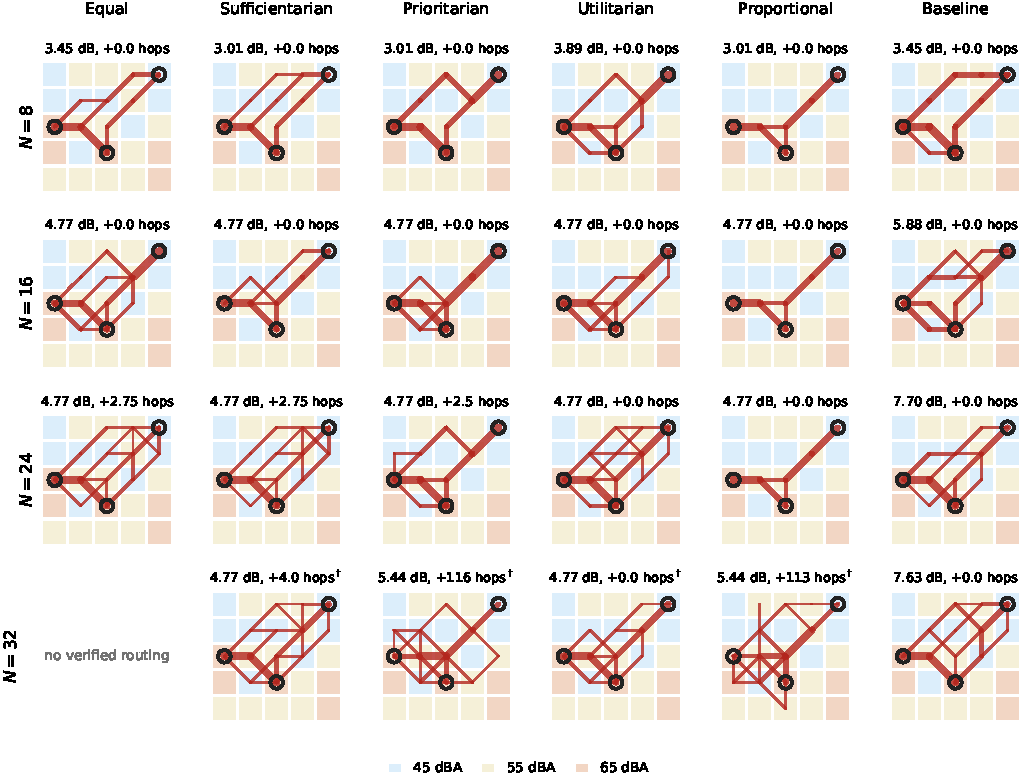
\includegraphics{figs/routes_grid.pdf}
\caption{The instance at four fleet sizes, one column per condition. Tiles are shaded by
ambient level, vertiports ringed, and each panel overlays every aircraft's path with line
width proportional to the aircraft on that leg, for one representative permutation.
Because the widths sum over the horizon, two panels can look alike while the routings
differ in \emph{when} each leg is flown. A dagger marks a cell that was harvested at the
budget horizon rather than proven.}
\label{fig:routes-grid}
\end{figure*}

\begin{figure*}[t]
\centering
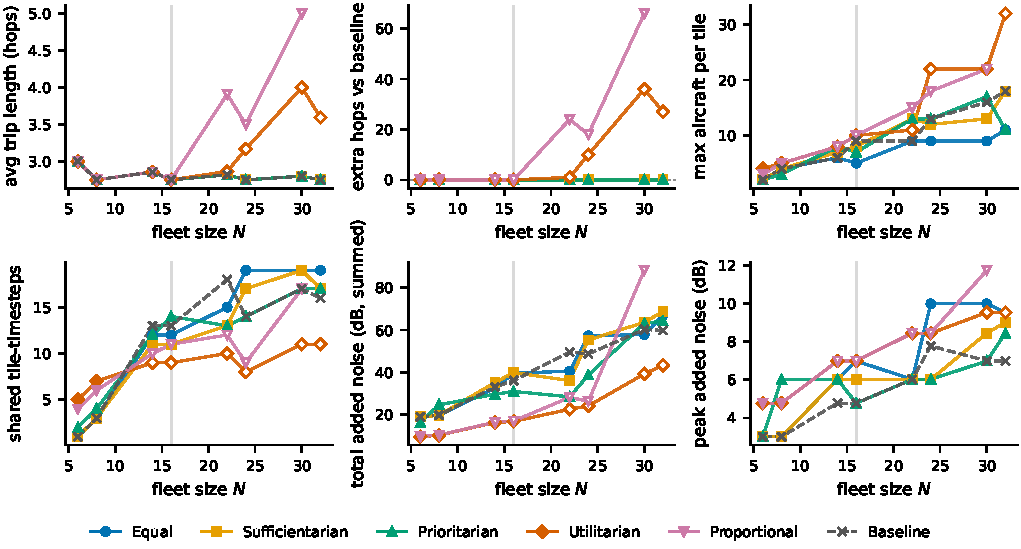
\includegraphics{figs/metric_vs_N.pdf}
\caption{Six metrics against fleet size. Each line runs through the mean of four
permutations of the aircraft list and the shaded band is their full range --- the
solver's indifference at that cell. Two conditions whose bands overlap are not separated
by anything the principle did. Lines join proven cells only; harvested cells appear as
isolated hollow markers, since a stopped search sits at an unknown distance from the
optimum and joining it to the curve would draw a trend out of how far the solver got.}
\label{fig:metric-vs-N}
\end{figure*}

\begin{table}[t]
\centering
\caption{How each principle responds to fleet size. \emph{From} is the smallest fleet at which the principle's routing differs from the no-fairness baseline by more than the permutation band at that cell; the arrow is whether that difference grows or shrinks above it. A dash means the principle never separates from the baseline on that metric, which is a property of the principle on this instance rather than a missing measurement.}
\label{tab:response}
\begin{tabular}{lllll}
\toprule
Principle & Congestion & Travel Time & Departure Delay & Added Noise \\
\midrule
Equal & -- & $-$ from $N{=}22$ & -- & $-$ from $N{=}22$ \\
Sufficientarian & -- & $-$ from $N{=}22$ & -- & $-$ from $N{=}22$ \\
Prioritarian & -- & $-$ from $N{=}22$ & -- & $-$ from $N{=}22$ \\
Utilitarian & -- & -- & $\uparrow$ from $N{=}22$ & $\uparrow$ from $N{=}22$ \\
Proportional & $-$ from $N{=}8$ & -- & $-$ from $N{=}22$ & $-$ from $N{=}22$ \\
\bottomrule
\end{tabular}
\end{table}


\begin{table}[t]
\centering
\caption{Routing under each principle as the fleet grows, on setup \texttt{D6\_protA} at an unlimited solver budget. \emph{+vs base} is total fleet hops above the no-fairness baseline at the same $N$; \emph{max/tile} the largest number of aircraft over one community at one timestep; \emph{shared} the tile-timesteps carrying two or more. Total added noise is the arithmetic dB sum the Utilitarian term minimises. A dagger marks a verified feasible routing whose optimality is unproven; every such number bounds the optimum rather than stating it.}
\label{tab:fleet-main}
\begin{tabular}{r l rr rr rr}
\toprule
$N$ & Condition & avg hops & +vs base & max/tile & shared & total dB & peak dB \\
\midrule
8 & Equal & 2.75 & 0 & 4 & 4 & 20.0 & 3.45 \\
8 & Sufficientarian & 2.75 & 0 & 4 & 3 & 19.6 & 3.01 \\
8 & Prioritarian & 2.75 & 0 & 4 & 5 & 17.0 & 3.01 \\
8 & Utilitarian & 2.75 & 0 & 3 & 5 & 20.4 & 3.89 \\
8 & Proportional & 2.75 & 0 & 5 & 5 & 11.6 & 3.01 \\
8 & Baseline & 2.75 & 0 & 4 & 4 & 19.4 & 3.45 \\
\midrule
16 & Equal & 2.75 & 0 & 8 & 14 & 35.0 & 4.77 \\
16 & Sufficientarian & 2.75 & 0 & 8 & 12 & 34.8 & 4.77 \\
16 & Prioritarian & 2.75 & 0 & 8 & 13 & 28.0 & 4.77 \\
16 & Utilitarian & 2.75 & 0 & 7 & 14 & 39.3 & 4.77 \\
16 & Proportional & 2.75 & 0 & 10 & 13 & 19.7 & 4.77 \\
16 & Baseline & 2.75 & 0 & 7 & 14 & 37.7 & 5.88 \\
\midrule
24 & Equal & 2.86 & 3 & 13 & 16 & 56.0 & 4.77 \\
24 & Sufficientarian & 2.86 & 3 & 13 & 16 & 56.0 & 4.77 \\
24 & Prioritarian & 2.85 & 2 & 12 & 17 & 40.3 & 4.77 \\
24 & Utilitarian & 2.75 & 0 & 11 & 18 & 53.9 & 4.77 \\
24 & Proportional & 2.75 & 0 & 14 & 16 & 29.0 & 4.77 \\
24 & Baseline & 2.75 & 0 & 12 & 15 & 47.9 & 7.70 \\
\midrule
32 & Sufficientarian & 2.88$^\dagger$ & 4$^\dagger$ & 17$^\dagger$ & 19$^\dagger$ & 73.0$^\dagger$ & 4.77$^\dagger$ \\
32 & Prioritarian & 6.38$^\dagger$ & 116$^\dagger$ & 25$^\dagger$ & 33$^\dagger$ & 114.9$^\dagger$ & 5.44$^\dagger$ \\
32 & Utilitarian & 2.75$^\dagger$ & 0$^\dagger$ & 16$^\dagger$ & 20$^\dagger$ & 61.5$^\dagger$ & 4.77$^\dagger$ \\
32 & Proportional & 6.28$^\dagger$ & 113$^\dagger$ & 25$^\dagger$ & 37$^\dagger$ & 118.3$^\dagger$ & 5.44$^\dagger$ \\
32 & Baseline & 2.75 & 0 & 16 & 17 & 55.2 & 7.63 \\
\bottomrule
\end{tabular}
\end{table}


% Generated and current, deliberately not \input: tables/reference.tex (the shipped
% default in three lines -- the one paragraph in IV-A covers it), tables/capacity.tex,
% figs/solve_time.pdf, figs/route_sharing.pdf, figs/noise_over_time.pdf, figs/floor.pdf.
% The same convention tables/caps.tex already follows. Re-add any if a reviewer asks.
